\chapter{Allocation of the labour force} \label{appendix-Allocation_of_labour}

This appendix details the allocation of the labour force. In our model, the size of the workforce is determined by the size of the urban wage premium. With a uniformly distributed population on a grid of streets, the workforce is
    
\begin{align}\label{eqn:N}
N=2\left(\frac{\omega}{c}\right)^2.    
\end{align}
This is the urban labour supply. Labour demand is determined by a dual process - one determining how many workers each firm has, and one determining how many firms there will be. 
In the standard mode of the firm, the size of the firm's workforce is chosen optimally by setting the value of the marginal product labour equal to the wage.
\begin{align}\label{eqn:opt}
w = P*\beta*AN^\gamma k^\alpha n.^{beta-1}    
\end{align}
where the wage is 
\begin{align}\label{eqn:w}
w=(1 + \text{overhead})(\omega + \psi).
\end{align}
and by the population through the agglomeration effect.  \ref{eqn:opt} determines the demand for labour.

\begin{figure}
    \centering
    %\includegraphics{}
    \caption{Firm size, population and wage}
    
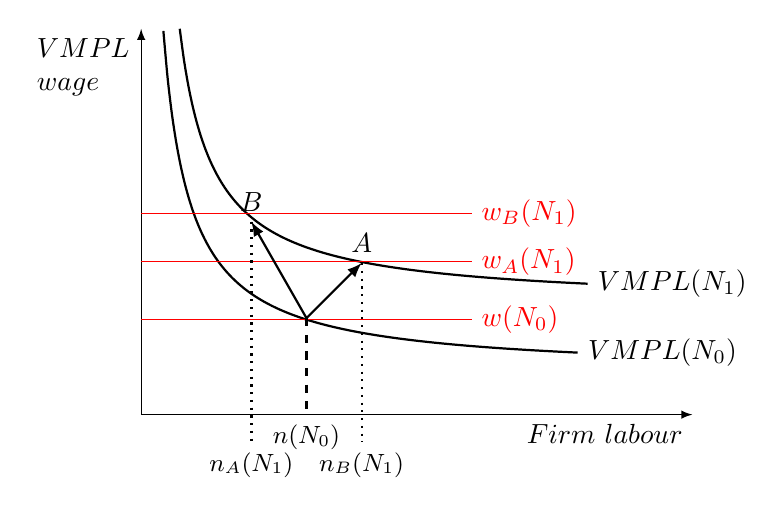
\begin{tikzpicture}[scale=.7, 
            my plot/.style={thick, smooth, samples=100, domain=0.4:10},
            plot2/.style={thick, smooth, samples=100, domain=0.1:9},
                    my grid/.style={opacity=0.5, 
                    every node/.style={black,opacity=1}},
                    my axis/.style={latex-latex}]
%\draw[my grid, step=.5cm,](0,0) grid (5,5);
 \draw[my axis] (0,7)node[below left, text width=1.2cm] {$VMPL$\\ $wage$} --(0,0)-- (10, 0) node[below left] {$Firm\ labour$}; %creates the axis 

 \draw[my plot, thick, domain=0.483:8] (0,0) plot ({\x-.08},{.75+3/\x})	node[right]{$VMPL(N_0)$}; 
 \draw[my plot, thick, domain=0.6:8] (0,0) plot ({\x+.1},{2+3/\x})node[right]{$VMPL(N_1)$};
% 
 \draw [thin, red ](0,1.73)--(6, 1.73)node[right]{$w(N_0)$};   %wage line
  \draw [thin, red ](0,2.77)--(6, 2.77)node[right]{$w_A(N_1)$};  
    \draw [thin, red ](0,3.65)--(6, 3.65)node[right]{$w_B(N_1)$};
      
\draw [thick,latex-latex](2,3.5)node[above]{$B$}--(3,1.75)--(4,2.75) node[above]{$A$};   %wage line
\draw[thick, dotted] (2,3.5)--(2,-.5)node[below]{\small$n_A(N_1)$};
\draw[thick,dashed] (3,1.75)--(3,0)node[below]{\small$n(N_0)$};
\draw[thick, dotted] (4,2.75)--(4,-.5)node[below]{\small$n_B(N_1)$};
\end{tikzpicture}
\label{fig:n_N_w}
\end{figure}

Depending on transport costs and other parameters, firm size may rise or fall as $N$ rises, as Figure~\ref{fig:n_N_w} shows. In the figure, $w_A$ results in rising firm size while $w_a$ results in a falling firm size. The wage selects a point on the VMPL curve but it also determines the  height of the curve, and the two processes are independent.

At the limit, the entire population might work for one firm, but in general, the number of firms will rise. The number of firms will depend on entry conditions and entrepreneurial expectations about profitability. For the housing market in our model, only $N$ matters and not the allocation of workers to firms.\footnote{In a more complex model firms might be distributed about the city and firm size could be significant.}

We can solve Equations~\ref{eqn:N} and \ref{eqn:opt} to find an explicit equilibrium relationship between $n$ and $N$. First solve Equation~\ref{eqn:w} for $n$, simplifying slightly by assuming constant factor proportions, i.e. that  $k=\kappa n$, in which case Equation~ \ref{eqn:opt} becomes: 
\begin{align}\label{eqn:opt1}
w   &= P*(\alpha+\beta)*AN^\gamma \kappa^\alpha n^{\alpha+\beta-1} \\   
n  &=\left(\frac{w}{P*(\alpha+\beta)*AN^\gamma \kappa^\alpha}\right)^{1-\alpha-\beta} \\
\end{align}

Let $(1-\alpha-\beta) = \zeta <1.$ Then:
\begin{align}
    &=\left(\frac{w}{P*(\alpha+\beta)*A \kappa^\alpha}\right)^\zeta N^{-\gamma\zeta }\\
    &=w^\zeta\left(\frac{1}{P*(\alpha+\beta)*A \kappa^\alpha}\right)^\zeta N^{-\gamma\zeta }\\
    &=w^\zeta*X*{N^{-\gamma}}^\zeta.
\end{align}
Where $X$ is a constant.

Now we use Equations~\ref{eqn:N} and \ref{eqn:w}to write $w$ as a function of $N$:
\[w=(1+overhead)(\psi+\frac{c}{\sqrt(2)}N^{.5}\]
so
\begin{align}
    n &= \left((1+overhead)(\psi+\frac{c}{\sqrt(2)}N^{.5}\right)^\zeta*X*N^{-\gamma\zeta }\\
  &= \left(a+b\sqrt(N)\right)^\zeta*X*N.^{-\gamma\zeta }   
\end{align}
In this simplified form it is easy to show that the slope of $n$ as $N$ changes is ambiguous, as the graphical treatment found.

Since none of our analysis depends on firm size, we can assume for convenience that firm size $n$ is constant and directly calculate demand for $N$ from
\[w  = P*(\alpha+\beta)*AN^\gamma \kappa^\alpha n^{\alpha+\beta-1}  \]

\begin{align}\label{fig:N_demand}
N   &= (\frac{n^\zeta P(\alpha+\beta)A\kappa^\alpha}{w})^\gamma  \nonumber\\
    &= C \left(\frac{P}{w}\right)^\gamma.
\end{align}
Equation~\ref{fig:N_demand} describes the population that would result in the firm choice of $n$ and $k$ being optimal. Since $\zeta$ is negative, larger  $n$ would call for a lower $N$ to achieve a value marginal product of labour equal to the wage.

%Demand for $N$ is downward sloping in the wage, as expected. Combined with the supply curve, Equation~\ref{eqn:N}, which slopes upward, we can be confident that the city has an equilibrium population. We don't know if it is stable, nor can we rule out the possibility of unlimited growth or collapse under some parameterisations.

% The profit function for the firm is achieved where  

